%\documentclass[18pt,oneside,a4paper, titlepage]{article}

%\usepackage[hidelinks]{hyperref}
%\usepackage[pdftex]{graphicx}
%\usepackage{lscape}
%\usepackage{pdflscape}

%\begin{document}

\newpage
	\section{Architectural Design}
		\subsection{Overview}
			This section deals with the specific description of the architectural choices made for the myTaxiService system. These decisions are supported by different diagrams, whose aim is to highlight and simplify the view of the components of the system, and explanations about the architectural styles adopted.
			\\In the first subsections there is a representation of the components of the system with diagrams. Here are presented the high level components and their interaction, with a brief definition of the functionalities of the three components individuated, then these are unfolded and there is a more specific description of the components, the interfaces and their relationships and features.\\
			The last subsection explains and justifies the architectural styles selected for the myTaxiService system, which consists in a client/server, event-based system, with a service-oriented, three-tier architecture (client, server and database). 
			
	
\newpage
		\subsection{High level components and their interaction}
		% here you can introduce the high level components of your architecture (in our basic example in the slides about design you find these in slide 7) and describe the main interaction between them (no details here. You can say why some components talk to each other, why, if the communication is synchronous or asynchronous, any other info you think is useful at this point). 
			\vspace{1cm}
			\begin{figure}[h]
				\centering
				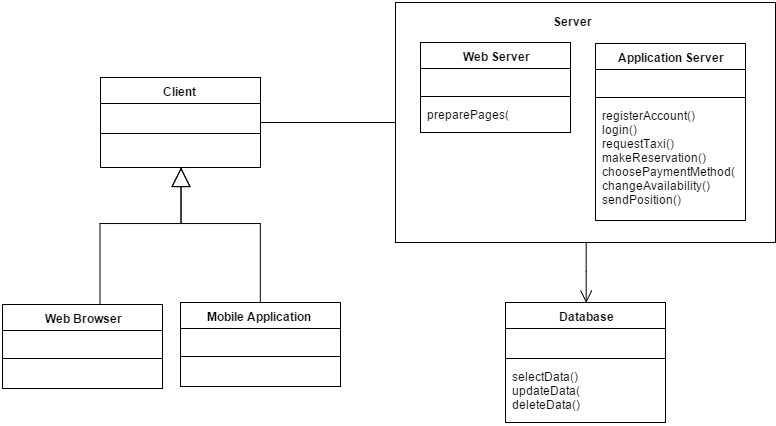
\includegraphics[scale=0.46]{Diagrams/HighLevelComp.png}
			\end{figure}
			\vspace{1cm}
			\begin{itemize}
				\item \textbf{Client}: this part runs on the client devices via a Web browser or the mobile application. It allows the users to insert and submit the data in the input forms, that are sent to the application server. On the other hand, the taxi drivers can send information about their availability to the server and the application client monitors their GPS position in order to move the taxi drivers to another queue if they change their area. 
				\item \textbf{Application Server}: this part runs on the JEE server. It is composed of a web server part, which always listens to all the clients requests and is responsible for the creation of the faces and pages of the client interfaces. The application server, instead, contains the logical part of the application, collecting and managing the information from the clients and the database. In fact, it analyses the data coming from the clients and, according to the requests, it modifies or asks for the required information stored in the database, then it is able to answer the client request, sending it the result.  
				\item \textbf{Database}: this part contains the database where all the application data are stored. It is not only accessed by the application server, but also by the administrators, who can, for example, directly add a taxi driver account to the database. 
			\end{itemize}	
			
	\newpage
		\subsection{Component view}
		% here you have a refinement of what you have in Section 4.B and identify sub-components. For instance, the diagram in slide 6 could be a diagram showing a  component view
		In the diagram below are showed the components that define the myTaxiService system architecture, which is composed by many subsystems and an external component which belongs to the database.\\ Starting from the left, in the first subsystem, the \textbf{Controller}, there are two components that manage the requests of the users and the payments.\\ The \textit{RequestManager} component manages all the logic of the requests, getting the information from the users and forwarding them to the designated taxi driver. As it deals with several tasks, he needs more than one interface to be implemented: \textit{RequestTaxiVisitor}, \textit{Notifications}, \textit{RequestTaxiPassenger} and \textit{MakeReservation} are the required interfaces for this component. It also relates with other components: it uses the \textit{PaymentManager} and the \textit{Data}, in order to complete its operations, and creates the \textit{ChoosePaymentMethod} interface, which is required by the \textit{PaymentManager}.\\
		The second subsystem is called \textbf{Functions}, as it provides the possible actions that the user can do while using the system. It is composed by four interfaces provided to the \textbf{Controller}: \textit{PaymentManager}, \textit{RequestTaxiPassenger}, \textit{MakeReservation} and \textit{Notifications}.\\
		This last interface can be accessed from the taxi driver mobile application to see the notifications of the requests, in fact it is produced by the \textit{TaxiDriverArea} interface.
		The \textit{RequestTaxiPassenger} and \textit{MakeReservation} interfaces, instead, are created by the \textit{PassengerArea} interface, which is part of the subsystem \textbf{Account} with \textit{TaxiDriverArea}. They are used by the passenger when he needs to request a taxi or make a reservation from his personal area.\\
		Another subsystem is the \textbf{AccountManager} whose main goal is to manage the access of the users, forwarding them to the proper designated area. The \textit{TaxiDriverAreaManager} requires the interface \textit{TaxiDriverArea}, which is provided by the \textit{TaxiDriverArea} interface in \textbf{Account}. The same relation is defined between the \textit{PassengerAreaManager} component and the \textit{PassengerArea}. The third component of this subsystem, the \textit{AccessManager}, which is responsible for the log in and the registration of the users, creates an instance of \textit{PassengerArea}, while requires the interface \textit{Access}.\\
		The last subsystem is the \textbf{Visitor}, which provides the interface \textit{Access} to the \textit{AccessManager} and another interface, \textit{RequestTaxi} to the \textit{RequestManager}. In fact, this subsystem represent the home page where the visitor can register or log in and request a taxi.
		
		
		\begin{landscape}
			\newpage
			\begin{figure}[!h]
				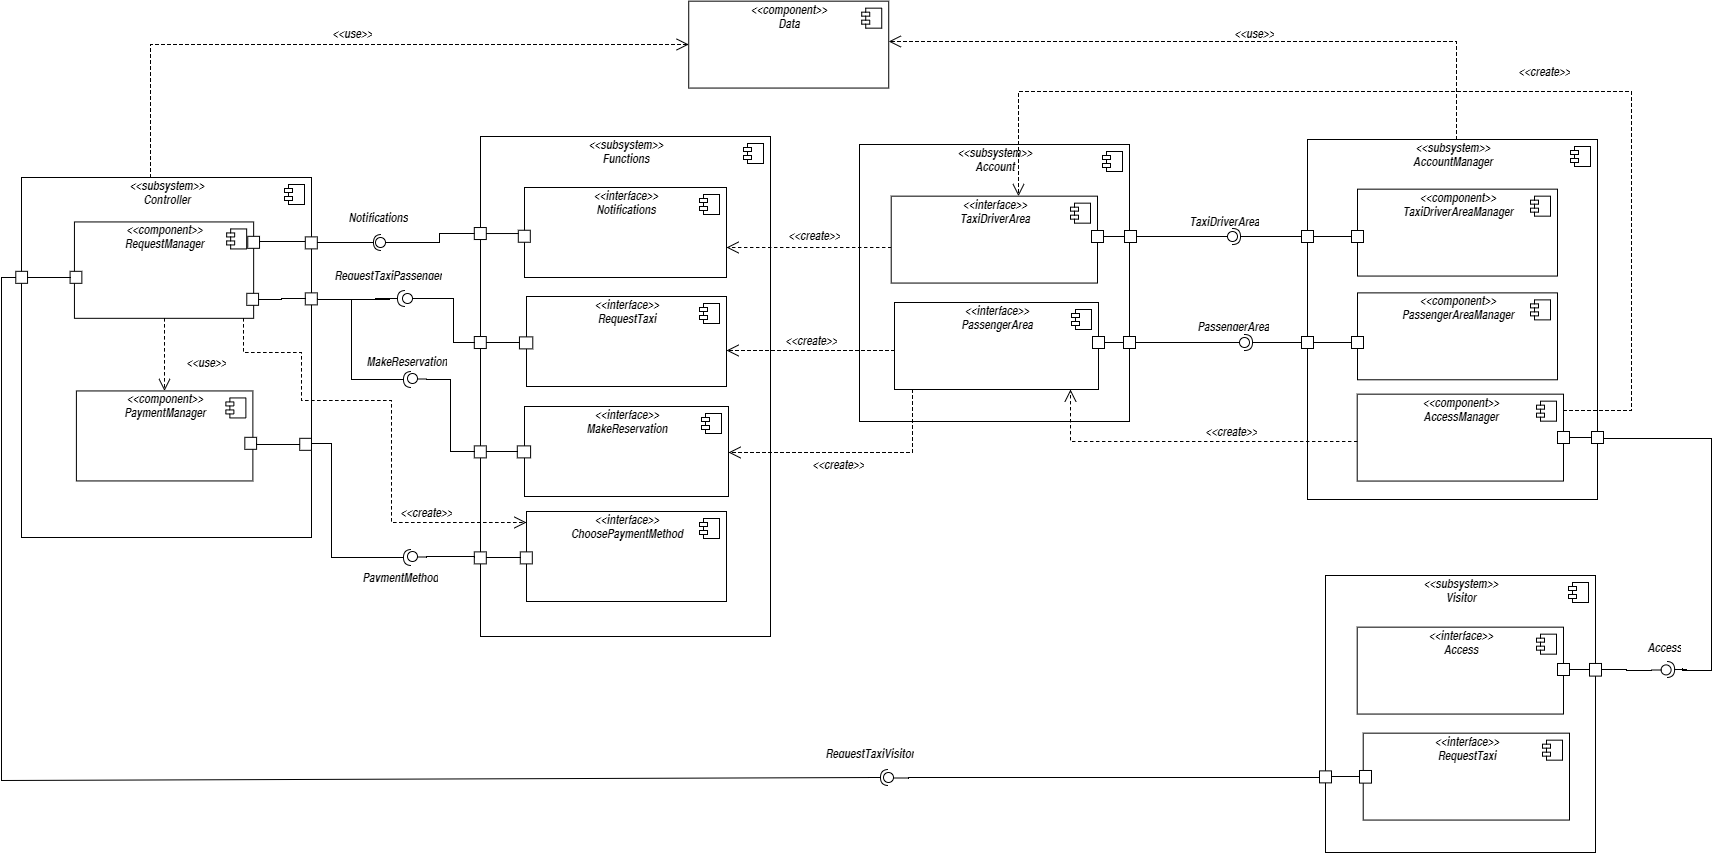
\includegraphics[scale=0.41]{Diagrams/componentDiagram.png}
			\end{figure}
		\end{landscape}
		
	\newpage	
		\subsection{Deployment view}
		% this is what you have in slide 8, that is, the identification of the artifact that need to be deployed to have the system working
		This diagram shows where the components presented in section 2.3 are deployed in the system.
		\vspace{0,7cm}
		\begin{figure}[h]
			\centering
			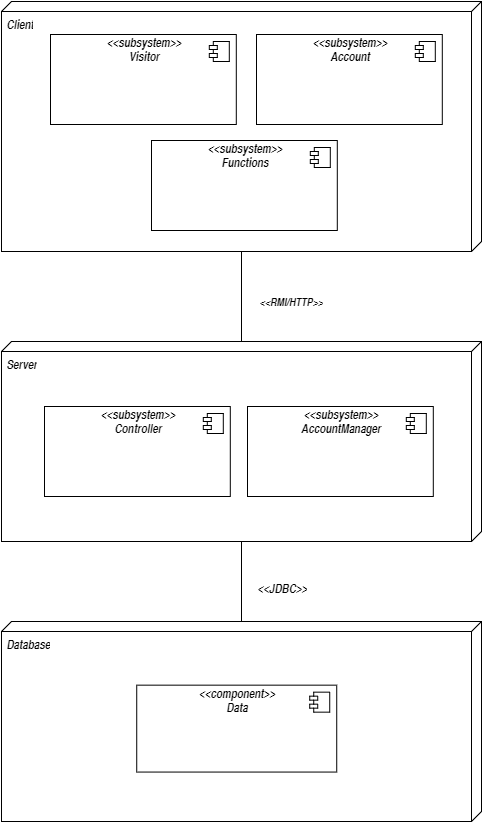
\includegraphics[scale=0.56]{Diagrams/deploymentDiagram.png}
		\end{figure}
	\newpage
		\subsection{Runtime view}
		%	You can use sequence diagrams to describe the way components interact to accomplish specific tasks typically related to your use cases
		% this is what you have in slide 9 plus sequence diagrams describing the way components behave in order to accomplish a certain activity
		This diagram depicts how components presented in section 2.3 works in order to execute the operations of the system.\\
		These kind of activities are shown also in the following sequence diagrams, here reported in order to show more in details how the components behave.
		\vspace{2cm}
			\begin{figure}[h]
				\centering
				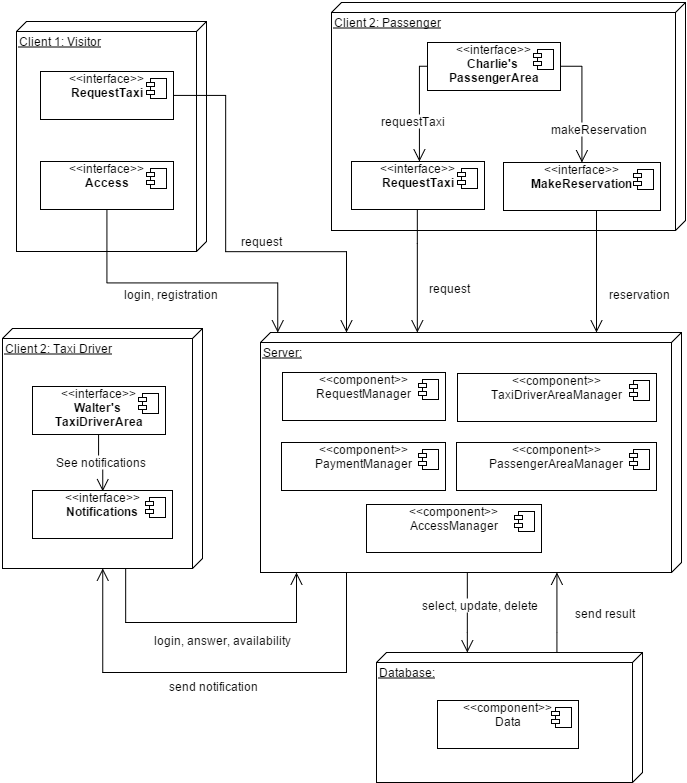
\includegraphics[scale=0.55]{Diagrams/RunTimeView.png}
			\end{figure}
		\begin{landscape}
			\newpage
				\begin{figure}[h]
					\centering
					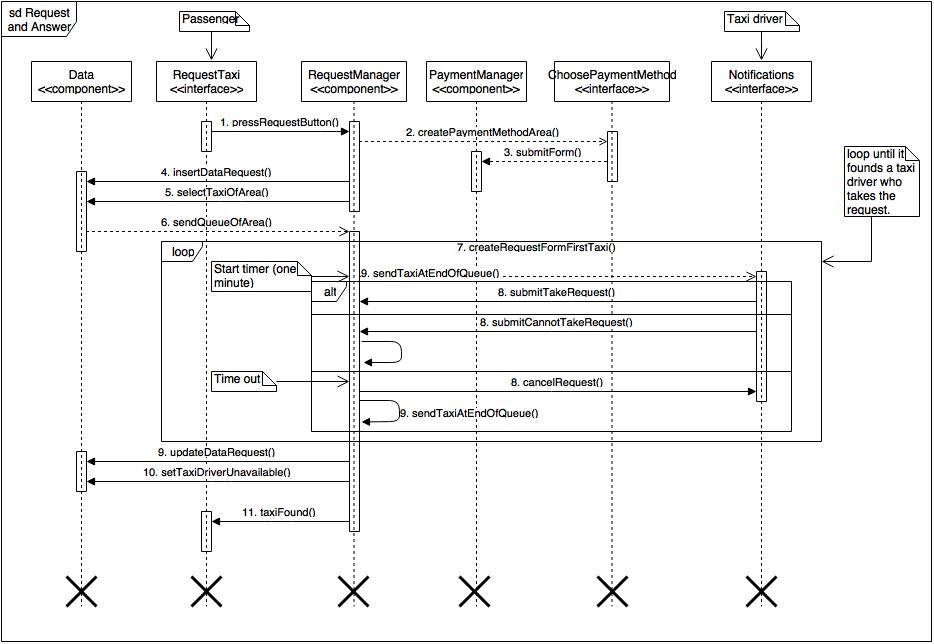
\includegraphics[scale=0.65]{Diagrams/SDRequest.jpg}
				\end{figure}
			\newpage
				\begin{figure}[h]
					\centering
					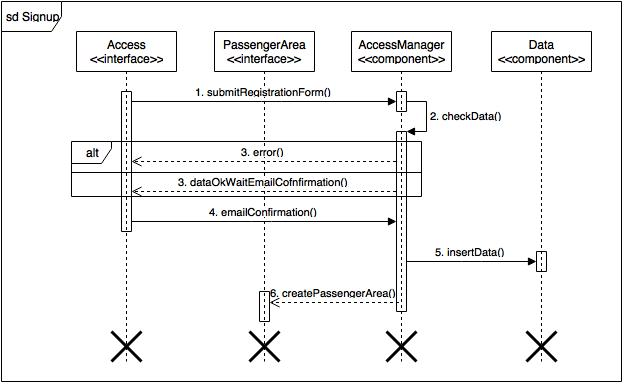
\includegraphics[scale=0.95]{Diagrams/SDSignup.jpg}
				\end{figure}
			\newpage
			\begin{figure}[h]
				\centering
				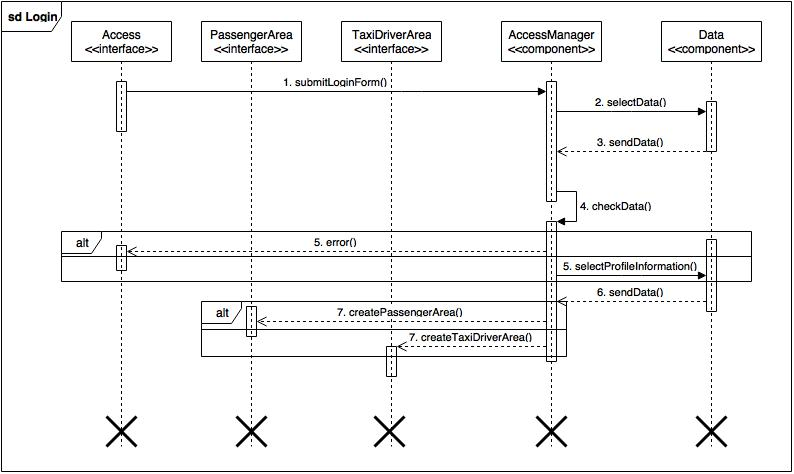
\includegraphics[scale=0.75]{Diagrams/SDLogin.jpg}
			\end{figure}
			\newpage
			\begin{figure}[h]
				\centering
				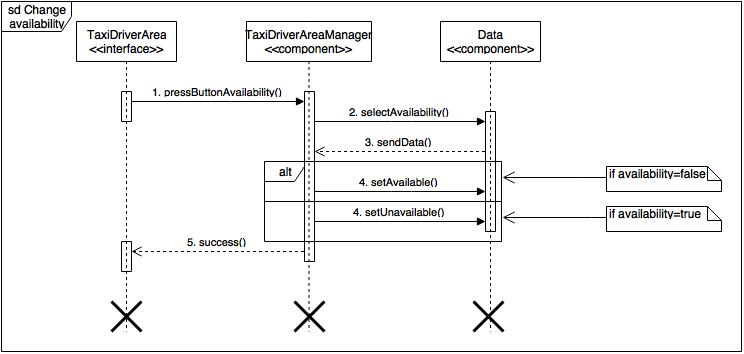
\includegraphics[scale=0.85]{Diagrams/SDAvailability.jpg}
			\end{figure}
		\end{landscape}
		
	\newpage
	\subsection{Component interfaces}
	% here you define the interfaces of your components, that is, which operations they offer to the external world, their meaning, any input and output parameter (name, possible set of values/type)
	Here is presented a list of the interfaces defined in the component diagram in section 2.3 and their functionalities.
	\begin{itemize}
		\item \textbf{Access.}
		This interface allows a generic user to log into the system as a passenger or as a taxi driver and allows the visitor to sign up. It requires the visitor to insert his personal information, e-mail address and password if he wants to register, otherwise only e-mail address and password to log in. \\ The inputs of the login as a passenger are:
		\begin{itemize} 
			\item[-] Email (String)
			\item[-] Password (String)
		\end{itemize}
		The inputs of the login as a taxi driver are:
		\begin{itemize} 
			\item[-] Email (String)
			\item[-] Password (String)
			\item[-] Code (String)
		\end{itemize} 
		The inputs of the registration are:
		\begin{itemize} 
			\item[-] Email (String)
			\item[-] Name (String)
			\item[-] Surname (String)
			\item[-] Password (String)
			\item[-] Phone number (String)
		\end{itemize}
		If the data entered are correct, the output is the redirection to the user personal area, otherwise an error message is displayed.
		\item \textbf{TaxiDriverArea.}
		This interface allows the taxi driver to see and modify his profile information, to change his availability and to see his position in the queue. The taxi driver has to insert new personal information if he wants to modify his profile or he can  press the availability button if he only needs to change his state.\\ The inputs of the edit profile form are:
		\begin{itemize} 
			\item[-] Email (String)
			\item[-] Name (String)
			\item[-] Surname (String)
			\item[-] Password (String)
			\item[-] Phone number (String)
		\end{itemize}
		The input of the availability button is true or false whether he wants to declare itself available or not.\\The output of this interface is the profile of the taxi driver with the position of the queue, the availability button and the notifications.
		\item \textbf{PassengerArea.}
		This interface allows the passenger to see and modify his profile information, to make a request and to make a reservation. The passenger has to provide new personal information if he wants to edit his profile, otherwise he can press the designated button, in order to make the request or the reservation.\\ The inputs of the edit profile form are:
		\begin{itemize} 
			\item[-] Email (String)
			\item[-] Name (String)
			\item[-] Surname (String)
			\item[-] Password (String)
			\item[-] Phone number (String)
		\end{itemize}
		The outputs are the profile of the passenger or the redirection to the screen of the request or of the reservation.
		\item \textbf{Notifications.}
		This interface consists of a panel that allows the taxi driver to see and to accept or decline the requests of the users. The input is \textit{accept} if he wants to take the request, \textit{decline} otherwise. If the taxi driver does not answer within one minute the input is automatically set to \textit{timeOut}.\\ The output is the history of the requests previously forwarded.
		\item \textbf{RequestTaxiVisitor.}
		This interface allows the visitor to make a request directly from the homepage. The input is his position in that moment, which is sent automatically from the user device when he presses the button.\\ The output is a waiting screen.
		\item \textbf{RequestTaxiPassenger.}
		This interface allows the passenger to make a request. The input is his position in that moment, which is sent automatically from the user device when he presses the button. \\The output is the redirection to the payment method panel. 
		\item \textbf{MakeReservation.}
		This interface allows the passenger to make a reservation by filling in a form.\\ Its inputs are:
		\begin{itemize} 
			\item[-] DepartureTime (Time)
			\item[-] Origin (String)
			\item[-] Destination (String)
		\end{itemize}
		The output is the redirection to the payment method panel.
		\newpage
		\item \textbf{PaymentMethod.}
		This interface allows the passenger to choose the payment method he prefers. The input is \textit{cash} if he wants to pay the taxi driver with cash, \textit{card} otherwise. If he chooses to pay with the credit card he needs to provide his credit card data if he has not done it yet. \\ The inputs of the credit card data form are: 
		\begin{itemize} 
			\item[-] CardType (String)
			\item[-] FirstName (String)
			\item[-] LastName (String)
			
			\item[-] CardNumber (int)
			\item[-] ExpirationDate (Date)
			\item[-] CVV (int)
		\end{itemize}
		The output is the redirection to the waiting screen.
	\end{itemize}
	\newpage
		\subsection{Selected architectural styles and patterns}
		%	Please explain which style/patterns you used, why and how
		Here are explained the architectural styles and patterns adopted.
		\begin{itemize}
			\item \textbf{Client/Server architecture.} The client/server architecture is the optimal solution for the myTaxiService system, as it is necessary to have a central system that listens, manages and forwards the requests of the different clients. There is a central server that contains the logic of the application and the clients are the users of the system, such as visitors, passengers and taxi drivers.
			\item \textbf{Three-tier architecture.} It has been adopted a three-tier architectural model, composed by thin client, application server and database.\\ This architecture is the best choice for our system, even if it has some cons, such as the complexity of the structure and the difficulty of set up and maintenance, it still has several pros. For example, it guarantees increased performance and great flexibility, useful if there will be any future change concerning the architecture. Moreover it is granted a great security level, thanks to the decoupling of logic, data and presentation, which is essential as the system deals with several personal data.
			\item \textbf{Event-based system.} The myTaxiService application is based on the event firing. \\It is necessary, in fact, that the system is reactive and is able to do different quick operations according to the action of the clients. For the myTaxiService system events can be requests and reservations, as long as change of availability state or the answer to a request. \\The users and the taxi drivers are registered to different events and expect to receive notifications about what they need, whether it is the arrival of a taxi or the requests of the users.\\ The events are asynchronous and based on a "send and forget" paradigm, where the system only cares for sending the notifications to the designated clients or doing the actions needed in response of the event triggered.
			\item  \textbf{Service-Oriented Architecture (SOA).} A service-oriented architecture is necessary if the system wants to be more flexible and expandable. In fact, the myTaxiService application needs to provide programmatic interfaces in order to be open to future implementations of additional services. This can be guaranteed with this architectural choice, which is based on the loose coupling of the services, allowing to easily add more functionalities, without starting from scratch when a change is needed, and to simplify the maintenance of the system.
		\end{itemize}
							
%\end{document}